\begin{figure}[!htbp]
    \centering
    \subfloat[Top view.]{
        \begin{tikzpicture}[
            dimension/.style={draw, <->, >=stealth, thin, dashed, gray},
            ext/.style={draw, gray, thin},
            center/.style={fill=gray, draw=none, circle, inner sep=0.8pt}
        ]
            \node[anchor=south west, inner sep=0] (image) at (0,0) {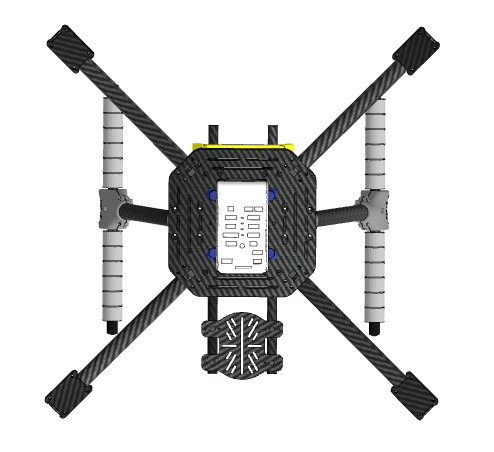
\includegraphics[width=0.34\textwidth]{Implementation/figures/drone_top_view.png}};
            \begin{scope}[x={(image.south east)},y={(image.north west)}]
                % Rotor centers (TL, TR, BL, BR)
                \coordinate (TL) at (0.142, 0.894);
                \coordinate (TR) at (0.844, 0.894);
                \coordinate (BL) at (0.142, 0.122);
                \coordinate (BR) at (0.844, 0.122);
                \node[center] at (TL) {};
                \node[center] at (TR) {};
                \node[center] at (BL) {};
                \node[center] at (BR) {};

                % Rotor spacing along the frame sides (0.348 m), horizontal
                \draw[ext] (0.142, 0.945) -- (0.142, 0.985);
                \draw[ext] (0.844, 0.945) -- (0.844, 0.985);
                \draw[dimension] (0.142, 0.968) -- (0.844, 0.968);
                \node[font=\tiny, fill=white, inner sep=1pt] at (0.493, 0.968) {$0.348\,\text{m}$};

                % Rotor spacing along the frame sides (0.348 m), vertical
                \draw[ext] (0.088, 0.894) -- (0.022, 0.894);
                \draw[ext] (0.088, 0.122) -- (0.022, 0.122);
                \draw[dimension] (0.035, 0.894) -- (0.035, 0.122);
                \node[font=\tiny, rotate=90, fill=white, inner sep=1pt] at (0.035, 0.508) {$0.348\,\text{m}$};

                % Rotor spacing along the diagonal (0.49 m)
                \draw[<->, >=stealth, thin, dashed, white] (TL) -- (BR);
                \node[font=\tiny, rotate=-45, fill=white, inner sep=1pt] at ($(TL)!0.19!(BR)$) {$0.49\,\text{m}$};
            \end{scope}
        \end{tikzpicture}
        \label{fig:x500_top}
    }
    \hfill
    \subfloat[Front view.]{
        \begin{tikzpicture}[
            dimension/.style={draw, <->, >=stealth, thin, dashed, gray},
            ext/.style={draw, gray, thin},
            center/.style={fill=gray, draw=none, circle, inner sep=0.8pt}
        ]
            \node[anchor=south west, inner sep=0] (image) at (0,0) {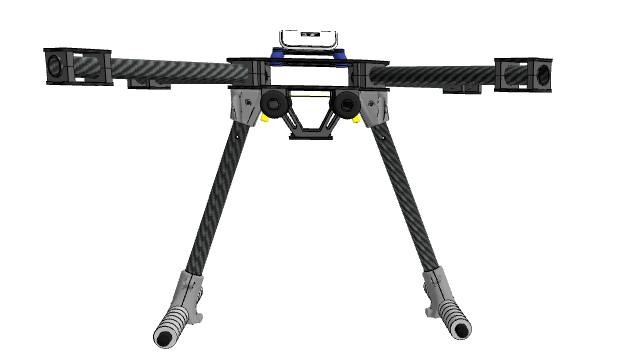
\includegraphics[width=0.52\textwidth]{Implementation/figures/drone_side_view.png}};
            \begin{scope}[x={(image.south east)},y={(image.north west)}]
                % Reference points: centre of the left motor mount and centres of the two feet
                \node[center] at (0.123, 0.814) {};
                \node[center] at (0.259, 0.061) {};
                \node[center] at (0.734, 0.086) {};

                % Height: from the ground (bottom of the feet) to the motor mounts (0.26 m)
                \draw[ext] (0.062, 0.814) -- (0.012, 0.814);
                \draw[ext] (0.235, 0.040) -- (0.012, 0.040);
                \draw[dimension] (0.025, 0.040) -- (0.025, 0.814);
                \node[font=\tiny, rotate=90, fill=white, inner sep=1pt] at (0.025, 0.427) {$0.26\,\text{m}$};

                % Base width: between the centres of the feet (0.264 m)
                \draw[ext] (0.259, 0.035) -- (0.259, -0.120);
                \draw[ext] (0.734, 0.060) -- (0.734, -0.120);
                \draw[dimension] (0.259, -0.100) -- (0.734, -0.100);
                \node[font=\tiny, fill=white, inner sep=1pt] at (0.4965, -0.100) {$0.264\,\text{m}$};
            \end{scope}
        \end{tikzpicture}
        \label{fig:x500_front}
    }
    \caption{x500 quadrotor layout.}
    \label{fig:x500_schematic}
\end{figure}